% architecture_minimal.tex — Minimal training diagram
\documentclass[border=4pt]{standalone}
\usepackage[T1]{fontenc}
\usepackage{amssymb}
\usepackage{tikz}
\usetikzlibrary{arrows.meta, positioning, calc, decorations.pathmorphing}

\definecolor{cFrz}{HTML}{BBDEFB}     \definecolor{cFrzB}{HTML}{1976D2}
\definecolor{cTrn}{HTML}{FFE0B2}     \definecolor{cTrnB}{HTML}{F57C00}
\definecolor{cData}{HTML}{C8E6C9}    \definecolor{cDataB}{HTML}{4CAF50}
\definecolor{cOu}{HTML}{F5F5F5}      \definecolor{cOuB}{HTML}{757575}
\definecolor{cLoss}{HTML}{FFCDD2}    \definecolor{cLossB}{HTML}{D32F2F}
\definecolor{cBP}{HTML}{C62828}

\begin{document}
\sffamily
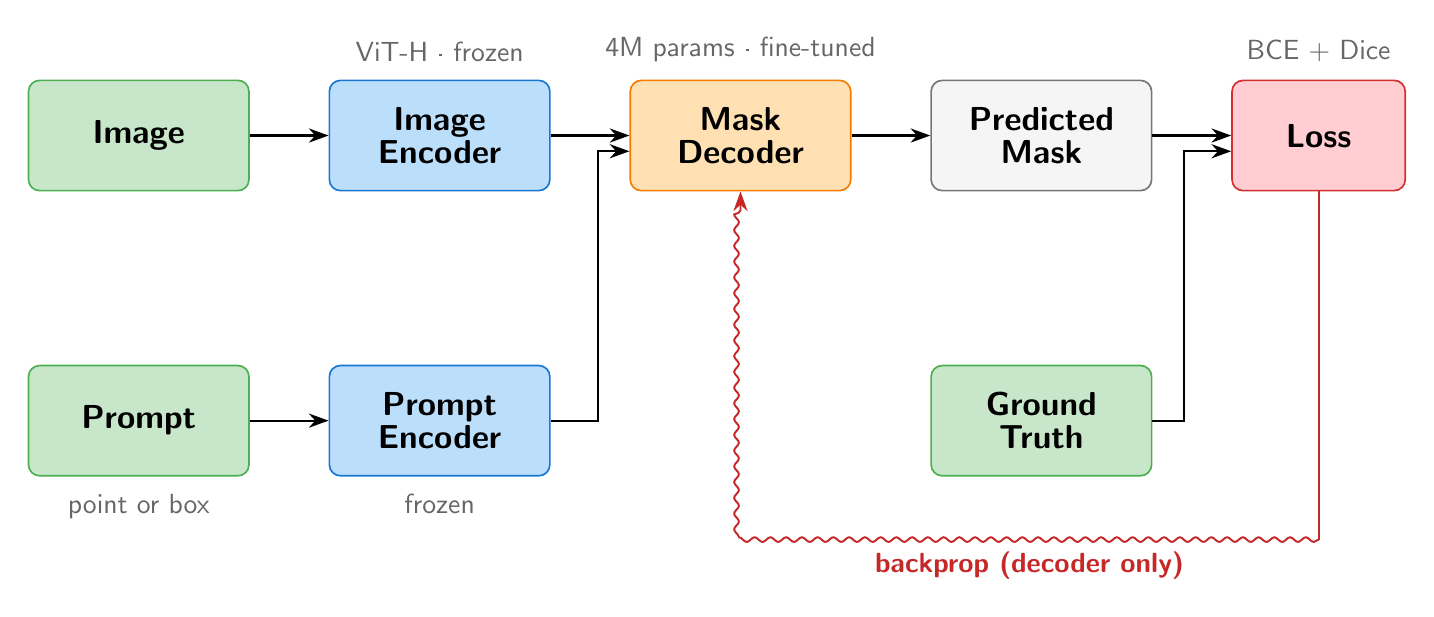
\begin{tikzpicture}[
    nd/.style={rounded corners=4pt, minimum height=14mm, minimum width=28mm,
               align=center, font=\large\sffamily\bfseries, line width=0.6pt},
    ndata/.style ={nd, fill=cData, draw=cDataB},
    nfrz/.style  ={nd, fill=cFrz,  draw=cFrzB},
    ntrn/.style  ={nd, fill=cTrn,  draw=cTrnB},
    nout/.style  ={nd, fill=cOu,   draw=cOuB},
    nlos/.style  ={nd, fill=cLoss, draw=cLossB, minimum width=22mm},
    ar/.style={-{Stealth[length=2.5mm,width=1.8mm]}, line width=0.8pt},
    sub/.style={font=\normalsize\sffamily, text=black!60, align=center},
]

% === ROW 1: Image → Encoder → Decoder → Predicted Mask ===
\node[ndata] (img) {Image};

\node[nfrz, right=10mm of img] (enc) {Image\\[-2pt]Encoder};
\node[sub, above=3pt of enc] {ViT-H \textperiodcentered\ frozen};

\node[ntrn, right=10mm of enc] (dec) {Mask\\[-2pt]Decoder};
\node[sub, above=3pt of dec] {4M params \textperiodcentered\ fine-tuned};

\node[nout, right=10mm of dec] (pred) {Predicted\\[-2pt]Mask};

\draw[ar] (img) -- (enc);
\draw[ar] (enc) -- (dec);
\draw[ar] (dec) -- (pred);

% === ROW 2: Prompt → Prompt Encoder → Decoder ===
\node[ndata, below=22mm of img] (prm) {Prompt};
\node[sub, below=3pt of prm] {point or box};

\node[nfrz, right=10mm of prm] (pe) {Prompt\\[-2pt]Encoder};
\node[sub, below=3pt of pe] {frozen};

\draw[ar] (prm) -- (pe);
\draw[ar, line width=0.8pt] (pe.east) -- ++(6mm,0) |- ([yshift=-2mm]dec.west);

% === GT below Predicted Mask, Loss below and right ===
\node[ndata, below=22mm of pred] (gt) {Ground\\[-2pt]Truth};

\node[nlos, right=10mm of pred] (loss) {Loss};
\node[sub, above=3pt of loss] {BCE + Dice};

\draw[ar] (pred) -- (loss);
\draw[ar] (gt.east) -- ++(4mm,0) |- ([yshift=-2mm]loss.west);

% === BACKPROP: Loss → down → left → up to Decoder ===
\coordinate (bpY) at ([yshift=-8mm]gt.south);

\draw[cBP, line width=0.7pt]
    (loss.south) -- (loss.south |- bpY);

\draw[cBP, line width=0.7pt,
      decorate, decoration={snake, amplitude=0.3mm, segment length=2mm,
                            post length=1.5mm},
      -{Stealth[length=2.5mm,width=1.8mm]}]
    (loss.south |- bpY) -- (dec.south |- bpY) -- (dec.south);

\node[font=\normalsize\sffamily\bfseries, text=cBP, anchor=north]
    at ($(dec.south |- bpY)!0.5!(loss.south |- bpY) + (0,-1pt)$)
    {backprop (decoder only)};

\end{tikzpicture}
\end{document}
